% !TEX encoding = UTF-8 Unicode
%!TEX root = thesis.tex

\newpage
\section{Background}

Prior to addressing the actual approach and implementation some concepts and terms have to be introduced. Firstly, the term \textit{security concept}, as it is used throughout the thesis, is being described. A definition of \textit{granularity levels} and system abstraction follows. Lastly, a section covers \textit{model transformations} and \textit{aggregation rules} on security attributes.

\subsection{Enterprise Security}
To define the term \textit{security concept} one has to look at the architecture of enterprises to understand the interconnectivity and interdependence between services, security being one of them.

\subsubsection{Enterprise Architecture}

Information systems tend to be a very complex artifacts that combine different views and requirements from various stakeholders of different backgrounds \cite{alex}. 

Software, IT platforms and IT related goals in general are covered in an \textit{Information System Architecture} (ISA). ISA does not take any business-driven influences into account and is therefore insufficient when describing the complex dependencies in corporations, especially when it comes to security as described in Subsection \ref{subsec:secarch}.   

\textit{Enterprise Architecture Modeling} tries to overcome such possible difficulties and combines IT related concerns with business and organizational goals and shows possible interrelationships. It therefore provides an approach for an improved understanding of complex enterprise processes \cite{earch}. The Federal Deposit Insurance Corporation (FDIC) published the results of an audit of its own implementation of E-Government principles \cite{fdicaudit} and their division of information technology in Figure \ref{fig:fdic} depicts the interrelations very well. 

\begin{figure}[H]
\centering
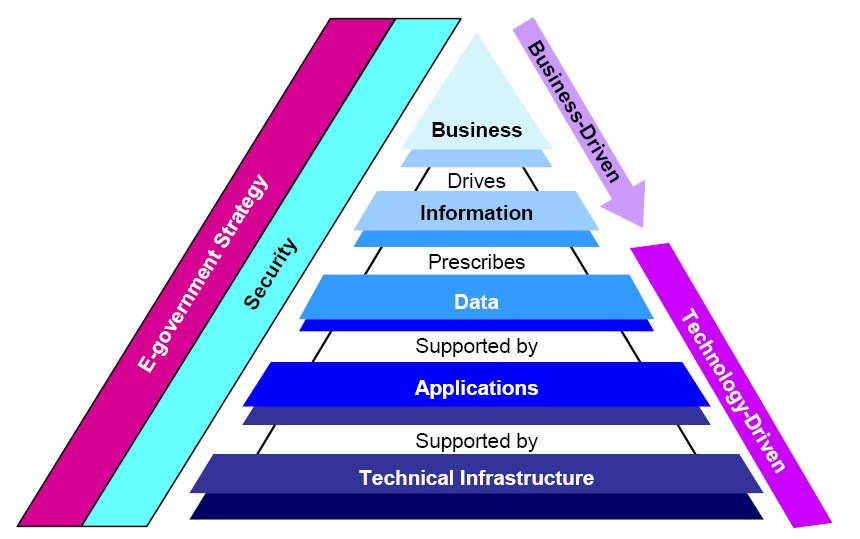
\includegraphics[width=0.6\textwidth]{pictures/fdic.jpg}
\caption{Division of Information Technology by FDIC}
\label{fig:fdic}
\end{figure}

\subsubsection{Security Architecture}
\label{subsec:secarch}

Information Security has often been merely an afterthought in corporations \cite{ansfederal} until a concept of a \textit{Security Architecture}, published in a whitepaper by The Gartner Group \cite{kreizman}, was introduced. 

\begin{figure}[H]
\centering
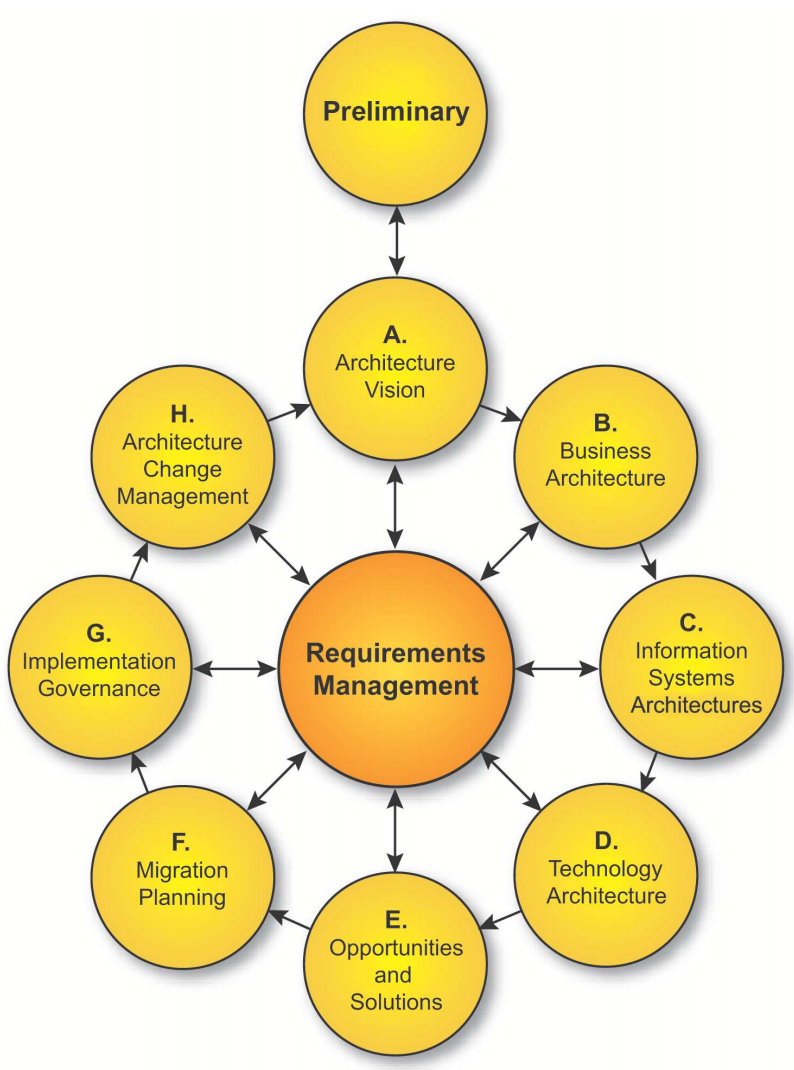
\includegraphics[width=0.6\textwidth]{pictures/togaf_overview.png}
\caption{Overview of the phases of TOGAF}
\end{figure}

\subsubsection{Common Criteria}
\subsubsection{Security Concept}

\subsection{Granularity Levels}

\subsection{Model Transformation}
\subsubsection{Aggregation rules}
